\subsection{Senkrechte (E-Feld) Polarisation (H-Feld parallel)}
\begin{center}
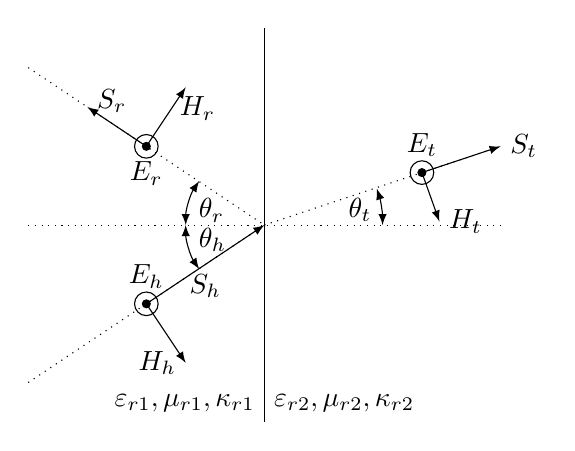
\begin{tikzpicture}
	\tikzset{cross/.style={cross out, draw=black, minimum size=2*(#1-\pgflinewidth), inner sep=0pt, outer sep=0pt},
		%     %default radius will be 1pt. 
		cross/.default={3.5pt}}
	%Kreuz
	\draw[dotted] (-3,0) -- (3,0);
	\draw[-] (0,2.5) -- (0,-2.5)                
	node[above right]   {$\varepsilon_{r2}, \mu_{r2}, \kappa_{r2}$}
	node[above left]    {$\varepsilon_{r1}, \mu_{r1}, \kappa_{r1}$};
	%Rücklaufende
	\draw[-latex] (-1.5,1) -- (-2.25,1.5)   node[right, yshift=.5ex]{$S_r$};
	\draw[-latex] (-1.5,1) -- (-1,1.75)     node[below, xshift=1ex] {$H_r$};
	\draw[-] (-1.5,1) circle (0.15)         node[below,yshift=-.5ex]{$E_r$};
	\draw[-,fill=black!100] (-1.5,1) circle (0.05);
	\draw[dotted] (-3,2) -- (0,0);
	\draw[latex-latex] (146:1) arc (146:180:1) 
	node[midway, right, yshift=-.7ex] {$\theta_r$};
	
	%Hinlaufende
	\draw[-latex] (-1.5,-1) -- (0,0)        node[below, midway]         {$S_h$};
	\draw[-latex] (-1.5,-1) -- (-1,-1.75)   node[left]                  {$H_h$};
	\draw[-] (-1.5,-1) circle (0.15)        node[above, yshift=.5ex]    {$E_h$};
	\draw[-,fill=black!100] (-1.5,-1) circle (0.05);
	\draw[dotted] (-3,-2) -- (0,0);
	\draw[latex-latex] (180:1) arc (180:214:1)
	node[midway, right, yshift=.7ex] {$\theta_h$};
	
	%Transmitierte
	\draw[-latex] (2,0.6666) -- (3,1)           node[right] {$S_t$};
	\draw[-latex] (2,0.6666) -- (2.2223,0.0448) node[right] {$H_t$};
	\draw[-] (2,0.6666) circle (0.15)           node[above, yshift=.5ex] {$E_t$};
	\draw[-,fill=black!100] (2,0.6666) circle (0.05);
	\draw[dotted] (0,0) -- (3,1);
	\draw[latex-latex] (0:1.5) arc (0:18:1.5)
	node[midway, left, yshift=-.3ex] {$\theta_t$};
	
\end{tikzpicture}
\end{center}



\[ \boxed{\texttt{mit } Z_{F0} = 120\pi \approx 377\si{\ohm}} \]
\begin{align*}
    Z_{Fn}                & = Z_{F0}\cdot\frac{1}{\sqrt{\varepsilon_{rn}}}            \\
    \frac{Z_{F1}}{Z_{F2}} & = \frac{\sqrt{\varepsilon_{r2}}}{\sqrt{\varepsilon_{r1}}}
\end{align*}
\[ n: \texttt{Brechungsindex} \quad ; \quad \theta_h = \theta_r\]
\begin{align*}
    \frac{\sin\theta_t}{\sin\theta_h} & = \frac{\lambda_2}{\lambda_1}= \frac{\beta_1}{\beta_2}= \frac{n_1}{n_2} \\
    \sin\theta_t                      & = \sqrt{\frac{\varepsilon_{r1}}{\varepsilon_{r2}}}\cdot \sin\theta_h
\end{align*}

\begin{itemize}
    \item magnetischer/elektrischer Reflexionsfaktor $[1]$
    \item magnetischer Transmissionsfaktor $[1]$
    \item elektrischer Transmissionsfaktor $[1]$
\end{itemize}
\begin{align*}
    r_s     & =  r_{e s} = r_{m s} =                                                                                                                                          \\
            & = \frac{Z_{F 2} \cdot \cos \theta_h-Z_{F 1} \cdot \cos \theta_t}{Z_{F 2} \cdot \cos \theta_h+Z_{F 1} \cdot \cos \theta_t}                                       \\
            & = \frac{\cos\theta_h-\sqrt{^{\varepsilon_{r2}}/_{\varepsilon_{r1}}-\sin^2\theta_h}}{\cos\theta_h+\sqrt{^{\varepsilon_{r2}}/_{\varepsilon_{r1}}-\sin^2\theta_h}} \\
    t_{m s} & = Z_{F 1} \cdot \frac{2 \cdot \cos \theta_h}{Z_{F 2} \cdot \cos \theta_h+Z_{F 1} \cdot \cos \theta_t}                                                           \\
            & = (1 - r_{s}) \cdot \dfrac{\cos \theta_h}{\cos \theta_t}                                                                                                        \\
            & = \frac{Z_{F1}}{Z_{F2}}\cdot t_{es}                                                                                                                             \\
    t_{e s} & = Z_{F 2} \cdot \frac{2 \cdot \cos \theta_h}{Z_{F 2} \cdot \cos \theta_h+Z_{F 1} \cdot \cos \theta_t}                                                           \\
            & = 1+r_{s}
\end{align*}

\begin{align*}
    E_{r} & = r_{s} \cdot E_{h}   \\
    E_{t} & = t_{e s} \cdot E_{h} \\
    H_{r} & = r_{s} \cdot H_{h}   \\
    H_{t} & = t_{m s} \cdot H_{h}
\end{align*}

\subsection{Parallel (E-Feld) Polarisation (H-Feld senkrecht)}
\begin{tikzpicture}
    \tikzset{cross/.style={cross out, draw=black, minimum size=2*(#1-\pgflinewidth), inner sep=0pt, outer sep=0pt},
        %     %default radius will be 1pt. 
        cross/.default={3.5pt}}
    %Kreunz
    \draw[dotted] (-3,0) -- (3,0);
    \draw[-] (0, 2.5) -- (0,-2.5) node[above right] {$\varepsilon_{r2}, \mu_{r2}, \kappa_{r2}$}
        node[above left] {$\varepsilon_{r1}, \mu_{r1}, \kappa_{r1}$};
 
    %Hinlaufende
    \draw[-latex] (-1.5,-1) -- (0,0) node[below, midway ]       {$S_h$};
    \draw[-latex] (-1.5,-1) -- (-2,-0.25) node[left, midway]    {$E_h$};
    \draw[-] (-1.5,-1) circle (0.15) node[below,yshift=-.5ex]   {$H_h$};
    \draw[-,fill=black!100] (-1.5,-1) circle (0.05);
    \draw[dotted] (-3,-2) -- (0,0);
    \draw[latex-latex] (180:1) arc (180:214:1)
        node[midway, right, yshift=.7ex] {$\theta_h$};

    %Rücklaufende
    \draw[-latex] (-1.5,1) -- (-2.25,1.5) node[right, yshift=.5ex]          {$S_r$};
    \draw[-latex] (-1.5,1) -- (-2,0.25) node[left, yshift=1ex, xshift=1ex]  {$E_r$};
    \draw[-] (-1.5,1) circle (0.15) node[above, yshift=.5ex]                {$H_r$};
    \draw[-,fill=black!100] (-1.5,1) circle (0.05);
    \draw[dotted] (-3,2) -- (0,0);
    \draw[latex-latex] (146:1) arc (146:180:1)
        node[midway, right, yshift=-.7ex] {$\theta_r$};
        
%    Rücklaufende Sattler
	%    Rücklaufende Sattler
	\draw[-] (-0.8,1.2) circle (0.15) node[right, xshift=.5ex]                {$H_r$};
	\draw(-0.8,1.2) node [cross] {};
 	\draw[-latex] (-0.8,1.2) -- (-0.3,1.95) node[left, yshift=1ex, xshift=1ex]  {$E_r$};
  	\draw[-latex] (-0.8,1.2) -- (-1.55,1.7) node[right, yshift=.5ex]          {$S_r$};

    %Transmitierte
    \draw[-latex] (2,0.6666) -- (3,1) node[right]                   {$S_t$};
    \draw[-latex] (2,0.6666) -- (1.7777,1.378)  node[right]         {$E_t$};
    \draw[-] (2,0.6666) circle (0.15) node[below, yshift=-0.5ex]    {$H_t$};
    \draw[-,fill=black!100] (2,0.6666) circle (0.05);
    \draw[dotted] (0,0) -- (3,1);
    \draw[latex-latex] (0:1.5) arc (0:18:1.5)
        node[midway, left, yshift=-.7] {$\theta_t$};

\end{tikzpicture}

\[ \boxed{\texttt{mit } Z_{F0} = 120\pi \approx 377\si{\ohm}} \]
\begin{align*}
    Z_{Fn}                & = Z_{F0}\cdot\frac{1}{\sqrt{\varepsilon_{rn}}}            \\
    \frac{Z_{F1}}{Z_{F2}} & = \frac{\sqrt{\varepsilon_{r2}}}{\sqrt{\varepsilon_{r1}}}
\end{align*}
\[ n: \texttt{Brechungsindex} \quad ; \quad \theta_h = \theta_r\]
\begin{align*}
    \frac{\sin\theta_t}{\sin\theta_h} & = \frac{\lambda_2}{\lambda_1}= \frac{\beta_1}{\beta_2}= \frac{n_1}{n_2} \\
    \sin\theta_t                      & = \sqrt{\frac{\varepsilon_{r1}}{\varepsilon_{r2}}}\cdot\sin\theta_h
\end{align*}

\begin{itemize}
    \item magnetischer/elektrischer Reflexionsfaktor $[1]$
    \item magnetischer Transmissionsfaktor $[1]$
    \item elektrischer Transmissionsfaktor $[1]$
\end{itemize}
\begin{align*}
    r_p     & =  r_{e p} = r_{m p} =                                                                                                                                                                                                      \\
            & = \frac{Z_{F 2} \cdot \cos \theta_t-Z_{F 1} \cdot \cos \theta_h}{Z_{F 2} \cdot \cos \theta_t+Z_{F 1} \cdot \cos \theta_h} =                                                                                                 \\
            & = \frac{\varepsilon_{r2}\cos\theta_h-\sqrt{\varepsilon_{r2}\varepsilon_{r1}-{\varepsilon_{r1}}^2\sin^2\theta_h}}{\varepsilon_{r2}\cos\theta_h+\sqrt{{\varepsilon_{r2}\varepsilon_{r1}-{\varepsilon_{r1}}^2\sin^2\theta_h}}} \\
    t_{m p} & = Z_{F 1} \cdot \frac{2 \cdot \cos \theta_h}{Z_{F 1} \cdot \cos \theta_h+Z_{F 2} \cdot \cos \theta_t}                                                                                                                       \\
            & = 1-r_{p}                                                                                                                                                                                                                   \\
    t_{e p} & = Z_{F 2} \cdot \frac{2 \cdot \cos \theta_h}{Z_{F 1} \cdot \cos \theta_h+Z_{F 2} \cdot \cos \theta_t}                                                                                                                       \\
            & = (1 + r_{p}) \cdot \dfrac{\cos \theta_h}{\cos \theta_t}                                                                                                                                                                    \\
            & = \frac{Z_{F2}}{Z_{F1}}\cdot t_{mp}
\end{align*}

\begin{align*}
    E_{r} & = r_{p} \cdot E_{h}   \\
    E_{t} & = t_{e p} \cdot E_{h} \\
    H_{r} & = r_{p} \cdot H_{h}   \\
    H_{t} & = t_{m p} \cdot H_{h} \\
\end{align*}
